\documentclass[11pt]{article}
\usepackage[T1]{fontenc}
\usepackage{lmodern}
\usepackage{microtype}
\usepackage{amsmath,amssymb,amsthm}
\usepackage{graphicx}
\usepackage{booktabs}
\usepackage{siunitx}
\usepackage{xcolor}
\usepackage{tikz}
\usetikzlibrary{positioning,arrows.meta}
\usepackage{hyperref}
\usepackage{cleveref}
\newtheorem{theorem}{Theorem}

\title{A Typical Paper}
\author{Benchmark}

\begin{document}
\maketitle

\section{Introduction}\label{sec:intro}
REVISION. This document loads the packages a typical paper uses. As
\cref{thm:main} shows, the method converges in \SI{3.2}{\second}.

\begin{theorem}\label{thm:main}
For all $n \in \mathbb{N}$, $\sum_{k=1}^{n} k = \frac{n(n+1)}{2}$.
\end{theorem}

\section{Results}
\begin{table}[h]
  \centering
  \begin{tabular}{lSS}
    \toprule
    Method & {Time (\si{\second})} & {Error} \\
    \midrule
    Baseline & 12.4 & 0.031 \\
    Ours     & 3.2  & 0.012 \\
    \bottomrule
  \end{tabular}
  \caption{Results.}
\end{table}

\begin{figure}[h]
  \centering
  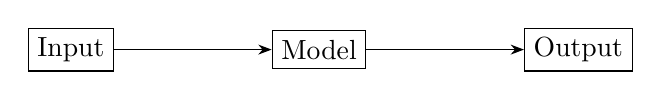
\begin{tikzpicture}[node distance=2cm, >=Stealth]
    \node[draw] (a) {Input};
    \node[draw, right=of a] (b) {Model};
    \node[draw, right=of b] (c) {Output};
    \draw[->] (a) -- (b);
    \draw[->] (b) -- (c);
  \end{tikzpicture}
  \caption{Pipeline.}
\end{figure}

\section{Conclusion}
See \cref{sec:intro} and \url{https://arxiv.org}.
\end{document}
